\documentclass[10pt,aspectratio=169]{beamer}

\usepackage[utf8]{inputenc}
\usepackage[T1]{fontenc}
\usepackage[french]{babel}
\usepackage{graphicx}
\usepackage{xcolor}
\usepackage{array}
\usepackage{tikz}
\usepackage{hyperref}

\usetikzlibrary{arrows.meta,positioning,shapes.geometric,shapes.multipart,calc}

\usetheme{Madrid}
\setbeamertemplate{navigation symbols}{}
\setbeamertemplate{caption}[numbered]

\definecolor{bookwiseGreen}{HTML}{0F766E}
\definecolor{bookwiseDark}{HTML}{042F2E}
\definecolor{bookwiseLight}{HTML}{ECFEFF}
\definecolor{softGray}{HTML}{F1F5F9}

\setbeamercolor{structure}{fg=bookwiseGreen}
\setbeamercolor{title}{fg=bookwiseDark}
\setbeamercolor{frametitle}{fg=white,bg=bookwiseGreen}
\setbeamercolor{block title}{fg=white,bg=bookwiseGreen}
\setbeamercolor{block body}{fg=black,bg=bookwiseLight}
\setbeamercolor{alerted text}{fg=bookwiseDark}

\hypersetup{
    pdftitle={Présentation PFA - BookWise},
    pdfauthor={Souhail Hajji, Dikra Benabdessadek}
}

\title[BookWise]{BookWise}
\subtitle{Conception et développement d'une application web de bibliothèque numérique}
\author{Souhail Hajji \and Dikra Benabdessadek}
\institute{École Marocaine des Sciences de l'Ingénieur \\ Encadrée par : Mme. Aarich Mounia}
\date{Année universitaire 2025/2026}

\begin{document}

\begin{frame}[plain]
    \centering
    
\includegraphics[width=0.78\textwidth,height=0.20\textheight,keepaspectratio]{assets/cover.png}

    \vspace{0.3cm}
    {\Large\bfseries Rapport de projet fin d'année\par}
    \vspace{0.18cm}
    {\large\bfseries BookWise\par}
    \vspace{0.12cm}
    {\normalsize Conception et développement d'une application web de bibliothèque numérique\par}

    \vspace{0.35cm}
    \begin{tabular}{>{\bfseries}r l}
        Réalisé par : & Souhail Hajji, Dikra Benabdessadek\\
        Encadrée par : & Mme. Aarich Mounia\\
        Filière : & Ingénierie Informatique et Réseaux\\
        Niveau : & 2ème année Cycle d'Ingénierie
    \end{tabular}

    \vfill
    {\small Année universitaire 2025/2026}
\end{frame}

\begin{frame}{Contexte général}
    \begin{columns}[T,onlytextwidth]
        \begin{column}{0.56\textwidth}
            \begin{block}{Idée du projet}
                BookWise est une plateforme web de bibliothèque numérique destinée à centraliser le catalogue, les commandes, les paiements et l'accès aux livres numériques.
            \end{block}

            \begin{itemize}
                \item Consultation d'un catalogue de livres publiés.
                \item Commande de livres avec paiement par virement bancaire.
                \item Validation administrative des preuves de paiement.
                \item Accès sécurisé à la lecture ou au téléchargement après approbation.
            \end{itemize}
        \end{column}
        \begin{column}{0.40\textwidth}
            \centering
            \begin{tikzpicture}
                \node[draw=bookwiseGreen, rounded corners=5pt, fill=bookwiseLight, minimum width=4.8cm, minimum height=0.85cm] (catalogue) {Catalogue};
                \node[draw=bookwiseGreen, rounded corners=5pt, fill=bookwiseLight, below=0.45cm of catalogue, minimum width=4.8cm, minimum height=0.85cm] (order) {Commande};
                \node[draw=bookwiseGreen, rounded corners=5pt, fill=bookwiseLight, below=0.45cm of order, minimum width=4.8cm, minimum height=0.85cm] (payment) {Preuve de paiement};
                \node[draw=bookwiseGreen, rounded corners=5pt, fill=bookwiseLight, below=0.45cm of payment, minimum width=4.8cm, minimum height=0.85cm] (library) {Bibliothèque personnelle};
                \draw[-{Stealth[length=2mm]}, thick] (catalogue) -- (order);
                \draw[-{Stealth[length=2mm]}, thick] (order) -- (payment);
                \draw[-{Stealth[length=2mm]}, thick] (payment) -- (library);
            \end{tikzpicture}
        \end{column}
    \end{columns}
\end{frame}

\begin{frame}{Problématique}
    \begin{block}{Constat}
        Les petites structures qui vendent ou diffusent des livres numériques utilisent souvent des outils séparés pour le catalogue, les commandes, les preuves de paiement et les fichiers.
    \end{block}

    \begin{columns}[T,onlytextwidth]
        \begin{column}{0.32\textwidth}
            \begin{block}{Gestion dispersée}
                Informations de livres, auteurs, catégories et commandes difficiles à suivre.
            \end{block}
        \end{column}
        \begin{column}{0.32\textwidth}
            \begin{block}{Validation manuelle}
                Les virements nécessitent une revue de preuve claire et traçable.
            \end{block}
        \end{column}
        \begin{column}{0.32\textwidth}
            \begin{block}{Accès numérique}
                Les fichiers doivent rester protégés jusqu'à l'approbation du paiement.
            \end{block}
        \end{column}
    \end{columns}
\end{frame}

\begin{frame}{Besoins fonctionnels}
    \small
    \begin{tabular}{|p{0.23\textwidth}|p{0.68\textwidth}|}
        \hline
        \textbf{Acteur} & \textbf{Fonctionnalités principales}\\
        \hline
        Lecteur & Créer un compte, se connecter, consulter le catalogue, commander des livres, déposer une preuve de paiement, suivre ses commandes, lire ou télécharger les livres achetés.\\
        \hline
        Administrateur & Gérer les livres, auteurs, catégories et utilisateurs, attribuer les rôles, consulter le tableau de bord, revoir les preuves et approuver ou rejeter les paiements.\\
        \hline
        Système & Authentifier les utilisateurs, contrôler les rôles, protéger les routes, sécuriser l'accès aux fichiers et maintenir les statuts de commande et de paiement.\\
        \hline
    \end{tabular}

    \vspace{0.35cm}
    \begin{block}{Assistance intelligente}
        Le chatbot aide les lecteurs sur le catalogue et peut proposer aux administrateurs des actions confirmables.
    \end{block}
\end{frame}

\begin{frame}{Besoins techniques}
    \begin{columns}[T,onlytextwidth]
        \begin{column}{0.48\textwidth}
            \begin{block}{Backend}
                \begin{itemize}
                    \item Java 21
                    \item Spring Boot 3.4.5
                    \item Spring MVC
                    \item Spring Data JPA
                    \item Maven
                \end{itemize}
            \end{block}
        \end{column}
        \begin{column}{0.48\textwidth}
            \begin{block}{Frontend et données}
                \begin{itemize}
                    \item Thymeleaf et Tailwind CSS
                    \item Spring Security avec JWT
                    \item PostgreSQL et H2 pour les tests
                    \item Chart.js pour le tableau de bord
                    \item Gemini API pour le chatbot
                \end{itemize}
            \end{block}
        \end{column}
    \end{columns}
\end{frame}

\begin{frame}{Conception du système : couches applicatives}
    \centering
    \begin{tikzpicture}[
        layer/.style={draw=bookwiseGreen, rounded corners=5pt, fill=bookwiseLight, minimum width=10.8cm, minimum height=0.85cm, align=center},
        side/.style={draw=bookwiseDark, rounded corners=5pt, fill=softGray, minimum width=3.0cm, minimum height=0.85cm, align=center, font=\small},
        arrow/.style={-{Stealth[length=2mm]}, thick}
    ]
        \node[layer] (ui) {Interface web : Thymeleaf, Tailwind CSS, Chart.js};
        \node[layer, below=0.38cm of ui] (controllers) {Contrôleurs Spring MVC : catalogue, auth, checkout, admin, chatbot};
        \node[layer, below=0.38cm of controllers] (services) {Services métier : commandes, paiements, bibliothèque, utilisateurs, sécurité};
        \node[layer, below=0.38cm of services] (repos) {Repositories Spring Data JPA};
        \node[layer, below=0.38cm of repos] (data) {PostgreSQL / H2 tests / stockage local des fichiers};

        \node[side, right=0.55cm of services] (security) {Spring Security\\JWT + rôles};
        \node[side, right=0.55cm of data] (gemini) {Gemini API\\assistant};

        \draw[arrow] (ui) -- (controllers);
        \draw[arrow] (controllers) -- (services);
        \draw[arrow] (services) -- (repos);
        \draw[arrow] (repos) -- (data);
        \draw[arrow] (security) -- (services);
        \draw[arrow] (services) -- (gemini);
    \end{tikzpicture}
\end{frame}

\begin{frame}{Diagrammes de cas d'utilisation}
    \centering
    \begin{columns}[T,onlytextwidth]
        \begin{column}{0.56\textwidth}
            \centering
            {\small Diagramme général\par}
            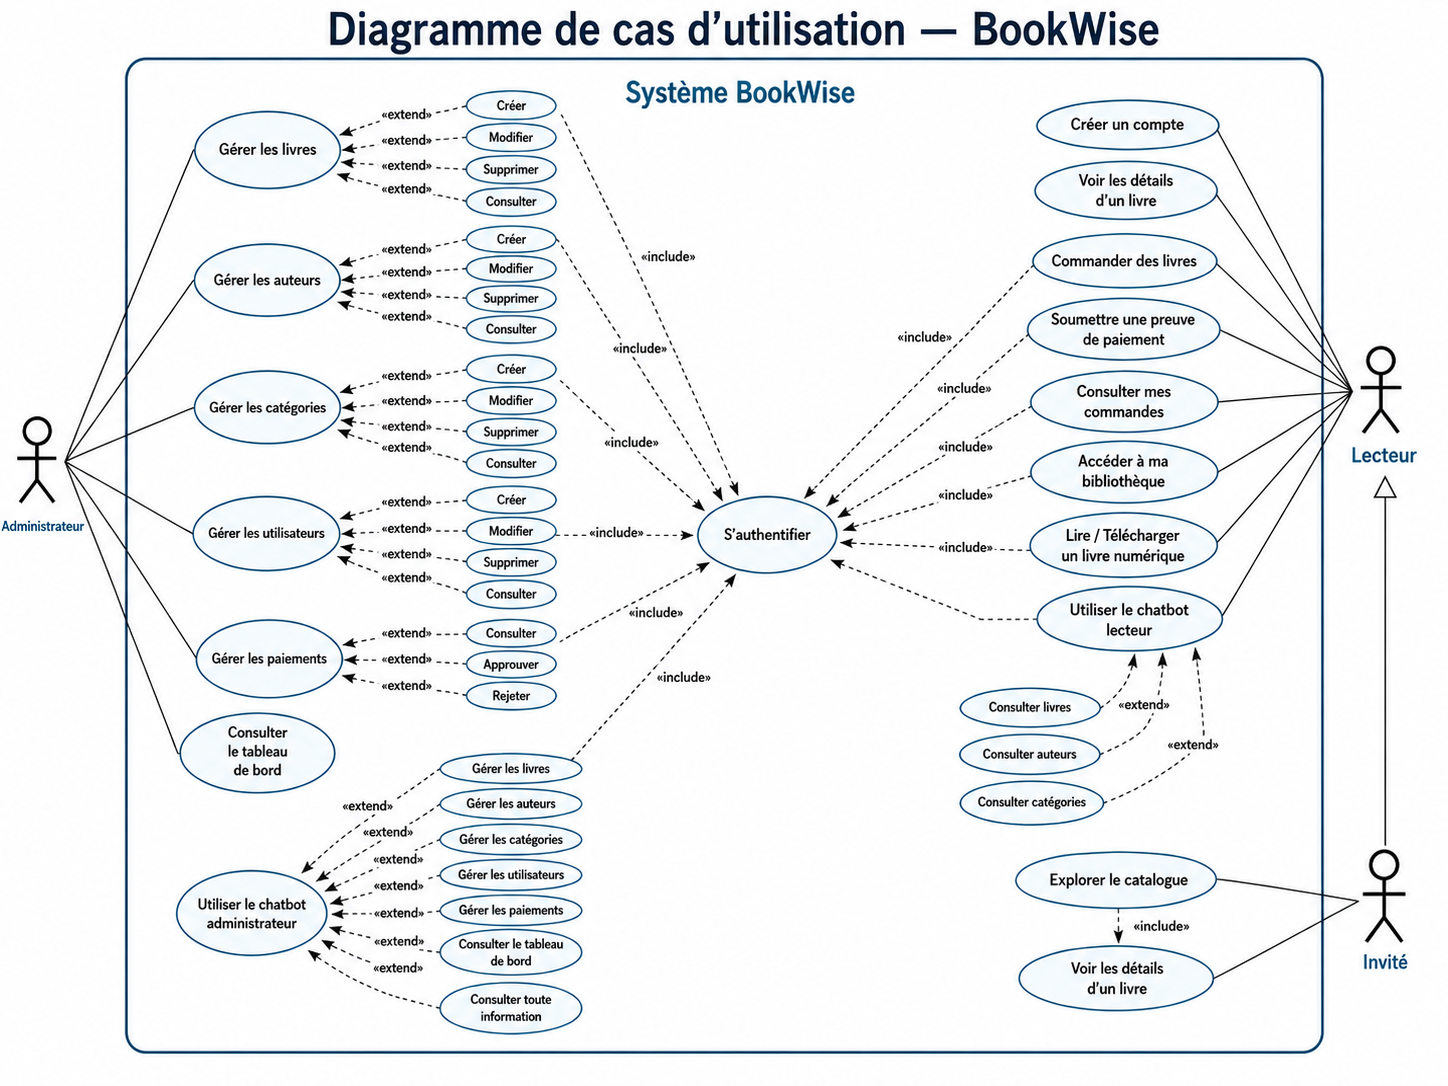
\includegraphics[width=\textwidth,height=0.72\textheight,keepaspectratio]{assets/usecase-general.png}
        \end{column}
        \begin{column}{0.42\textwidth}
            \centering
            {\small Lecteur\par}
            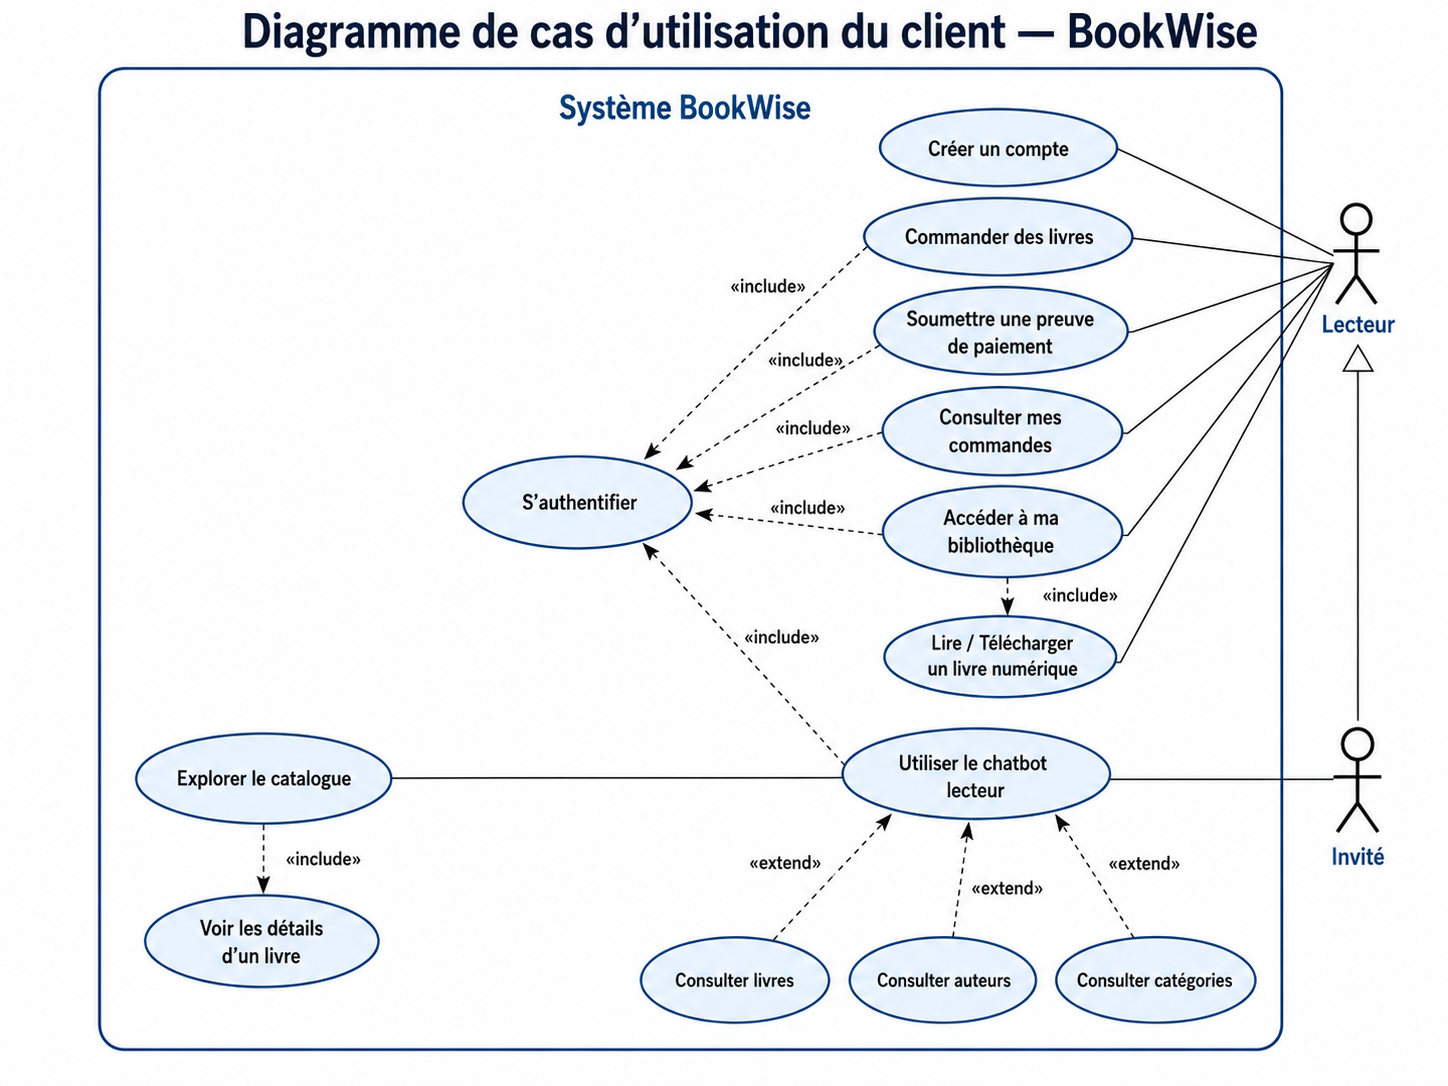
\includegraphics[width=\textwidth,height=0.32\textheight,keepaspectratio]{assets/usecase-client.png}

            \vspace{0.2cm}
            {\small Administrateur\par}
            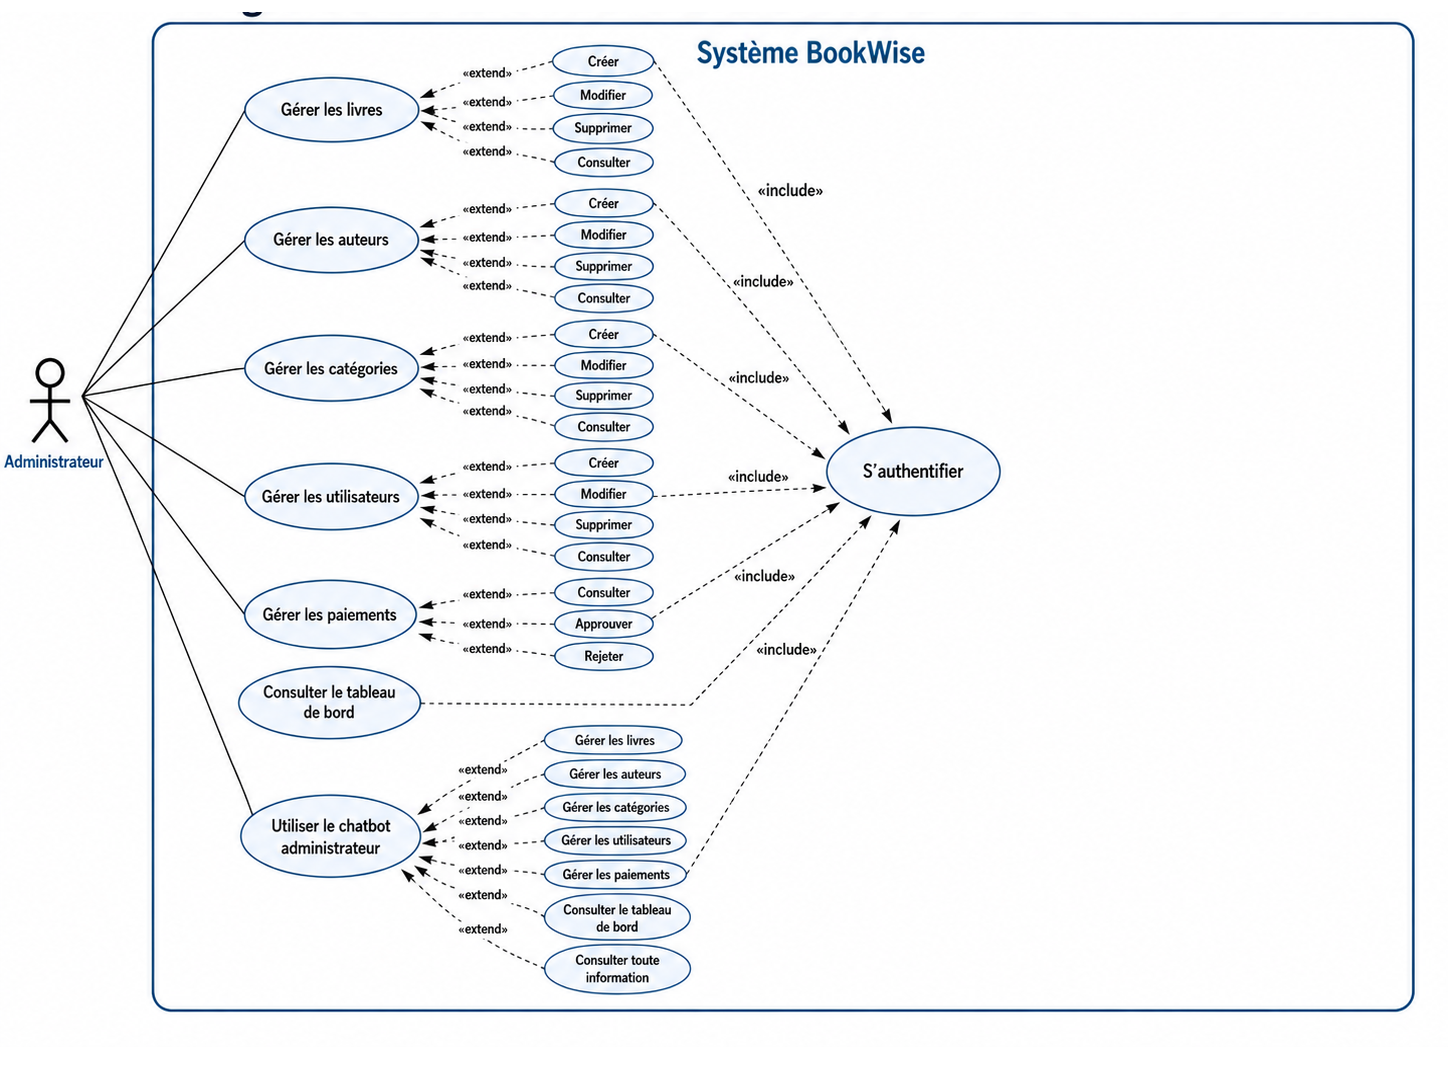
\includegraphics[width=\textwidth,height=0.32\textheight,keepaspectratio]{assets/usecase-admin.png}
        \end{column}
    \end{columns}
\end{frame}

\begin{frame}{Diagramme de classes}
    \centering
    \resizebox{0.98\textwidth}{!}{
    \begin{tikzpicture}[
        class/.style={draw=bookwiseGreen, rectangle split, rectangle split parts=2, fill=bookwiseLight, text width=2.75cm, align=left, font=\scriptsize},
        rel/.style={-{Stealth[length=2mm]}, thick}
    ]
        \node[class] (user) at (0,0) {
            \textbf{User}
            \nodepart{second}
            fullName\\email\\role
        };
        \node[class] (order) at (4.1,0) {
            \textbf{PurchaseOrder}
            \nodepart{second}
            totalAmount\\currency\\status
        };
        \node[class] (payment) at (8.2,0) {
            \textbf{Payment}
            \nodepart{second}
            method\\status\\receiptFileName
        };
        \node[class] (item) at (4.1,-2.7) {
            \textbf{OrderItem}
            \nodepart{second}
            unitPriceAmount\\quantity
        };
        \node[class] (book) at (8.2,-2.7) {
            \textbf{Book}
            \nodepart{second}
            title\\isbn\\priceAmount\\published
        };
        \node[class] (file) at (12.3,-2.7) {
            \textbf{BookFile}
            \nodepart{second}
            fileName\\storageKey\\fileType
        };
        \node[class] (author) at (6.1,-5.3) {
            \textbf{Author}
            \nodepart{second}
            fullName\\biography
        };
        \node[class] (category) at (10.3,-5.3) {
            \textbf{Category}
            \nodepart{second}
            name\\description
        };

        \draw[rel] (user) -- node[above,font=\scriptsize]{1..*} (order);
        \draw[rel] (order) -- node[above,font=\scriptsize]{1..1} (payment);
        \draw[rel] (order) -- node[left,font=\scriptsize]{1..*} (item);
        \draw[rel] (item) -- node[above,font=\scriptsize]{*..1} (book);
        \draw[rel] (book) -- node[above,font=\scriptsize]{1..*} (file);
        \draw[rel] (book) -- node[left,font=\scriptsize]{*..*} (author);
        \draw[rel] (book) -- node[right,font=\scriptsize]{*..*} (category);
    \end{tikzpicture}}
\end{frame}

\end{document}
